% Source of gamedepth-pipeline.pdf (compile with pdflatex).
\documentclass[tikz,border=1pt]{standalone}
\usepackage{lmodern}
\usetikzlibrary{positioning,arrows.meta,calc}
\begin{document}
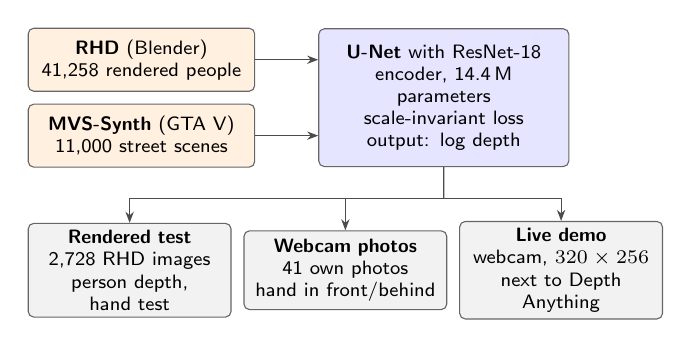
\begin{tikzpicture}[
  font=\sffamily\scriptsize,
  box/.style={draw=black!60, rounded corners=2pt, align=center, inner sep=2.5pt},
  data/.style={box, fill=orange!12, text width=27mm, minimum height=8mm},
  net/.style={box, fill=blue!10, text width=30mm, minimum height=17.5mm},
  test/.style={box, fill=black!5, text width=24mm, minimum height=10mm},
  arr/.style={-{Stealth[length=4pt]}, black!70}]
  \node[data, anchor=north west] (rhd) at (0,0) {\textbf{RHD} (Blender)\\41{,}258 rendered people};
  \node[data, below=1.5mm of rhd] (gta) {\textbf{MVS-Synth} (GTA~V)\\11{,}000 street scenes};
  \node[net, anchor=west] (unet) at ($(rhd.east)!0.5!(gta.east)+(8mm,0)$)
    {\textbf{U-Net} with ResNet-18\\encoder, 14.4\,M parameters\\scale-invariant loss\\output: log depth};
  \draw[arr] (rhd.east) -- (unet.west |- rhd.east);
  \draw[arr] (gta.east) -- (unet.west |- gta.east);
  \node[test, anchor=north west] (t1) at ($(gta.south west)+(0,-7mm)$)
    {\textbf{Rendered test}\\2{,}728 RHD images\\person depth, hand test};
  \node[test, right=1.5mm of t1] (t2) {\textbf{Webcam photos}\\41 own photos\\hand in front/behind};
  \node[test, right=1.5mm of t2] (t3) {\textbf{Live demo}\\webcam, $320\times256$\\next to Depth Anything};
  \coordinate (bus) at ($(unet.south)!0.5!(unet.south |- t2.north)$);
  \draw[black!70] (unet.south) -- (bus);
  \foreach \t in {t1,t2,t3} \draw[arr] (bus) -| (\t.north);
\end{tikzpicture}
\end{document}
